\documentclass{article}
\usepackage{iclr2027_conference,times}

% Optional math commands from https://github.com/goodfeli/dlbook_notation.
\input{math_commands.tex}

\usepackage{amsmath,amssymb}
\usepackage{booktabs}
\usepackage{graphicx}
\usepackage{array}
\usepackage{multirow}
\usepackage{xcolor}
\usepackage{hyperref}
\usepackage{microtype}
\usepackage{float}

\hypersetup{
  colorlinks=true,
  linkcolor=blue,
  citecolor=blue,
  urlcolor=blue
}

\title{Parallel Causal Associative Fields:\\
Gated Sparse Memory for Long-Context Language Modeling}

\author{Anonymous Authors \\
Affiliation \\
Address \\
\texttt{email}
}

\newcommand{\fix}{\marginpar{FIX}}
\newcommand{\new}{\marginpar{NEW}}

%\iclrfinalcopy % Uncomment for camera-ready version, but leave commented out for submission.

\begin{document}
\maketitle

\begin{abstract}
Transformers achieve strong language modeling performance by providing direct
token-to-token communication paths, but causal self-attention scales
quadratically with context length. Recurrent and state-space models reduce this
cost, yet compress history into sequentially updated fixed-size states. This
paper studies a third primitive: a parallel content-addressed memory over causal
successor records. The proposed Parallel Causal Associative Field (PCAF) writes
local records from a context window into hash buckets, retrieves a bounded
candidate set for the current query, forms a sparse cache distribution over
successor tokens, and mixes that cache with a parametric local language model
through a learned gate. The resulting model maintains sparse long-context access
while avoiding a single fixed recurrent state bottleneck.
We evaluate PCAF primarily on the large-scale WikiText-103 corpus using a
distributed Google Cloud TPU v4-32 pod. PCAF-context reaches 95.49 perplexity
at 38.92~M~tok/s, compared with 311.40 perplexity at 7.16~M~tok/s for the
dense Transformer baseline---a 5.4$\times$ throughput advantage alongside a
3.3$\times$ reduction in perplexity. On the semantic-routing ablation,
PCAF-context (context token-hash routing) outperforms PCAF-semantic (95.49
vs.\ 102.84 perplexity at $T{=}2048$), establishing discrete hash routing as
the stronger design choice. Supplementary single-GPU controlled ablations on
WikiText-2 using an NVIDIA RTX 3060 confirm that both the associative cache and
the learned gate are necessary: removing the cache degrades perplexity from
210.7 to 261.6 at $T{=}2048$, and replacing the learned gate with a fixed
mixture degrades perplexity to 247.0.
\end{abstract}

%%
%% 1. INTRODUCTION
%%
\section{Introduction}

Modern sequence models face a fundamental tension between memory access breadth
and computational cost. Self-attention grants each token a direct path to every
preceding token, a property that underlies the strong empirical performance of
Transformer-based language models
\citep{vaswani2017attention,bahdanau2015attention}. This direct access is
expensive: a causal attention layer over a length-$T$ sequence requires
$O(T^2 d)$ operations per layer, limiting practical context lengths under
memory and time constraints. Numerous strategies have been proposed to reduce
this cost. Sparse attention methods such as Longformer, BigBird, and the Sparse
Transformer restrict the attention graph to structured subsets of token pairs
\citep{beltagy2020longformer,zaheer2020bigbird,child2019sparsetransformer}.
Linear attention approximates the softmax kernel to achieve $O(T)$ per-layer
complexity \citep{katharopoulos2020linearattn}. Recurrent architectures based
on structured state spaces—most notably S4 and Mamba—achieve linear-time
sequence processing through selective state updates
\citep{gu2021s4,gu2023mamba}. Each of these approaches makes a distinct
trade-off: sparse attention limits the communication graph, linear attention
approximates the full attention matrix, and recurrent state-space models must
propagate long-range information through compressed fixed-dimensional states.

The motivation of this work is to disentangle two roles that are typically
conflated within the attention mechanism: \emph{memory addressing} and
\emph{value resolution}. Rather than constructing dense token-to-token
interactions, PCAF writes a sparse associative memory of causal records and
performs a bounded read from that memory. This read behaves analogously to a
neural cache \citep{grave2016continuous,khandelwal2019knn}, but is trained
jointly with a local parametric model and implemented as a parallel hash-bucket
primitive rather than an external nearest-neighbor index. The design draws
inspiration from memory-augmented neural networks
\citep{weston2015memory,sukhbaatar2015end2end} and from retrieval-augmented
language models \citep{borgeaud2022retro,izacard2022atlas}, but operates
\emph{within} a single context window without an external corpus.

The central empirical question is practical: can a simple associative memory
recover useful long-context signal without paying the cost of dense attention?
All models evaluated use the same WikiText-2 corpus, tokenizer, vocabulary
size, sampled windows, training-step budget, and evaluation protocol.
PCAF-context is compared against dense attention, sliding-window attention,
global-local sparse attention, and ablations that remove either the cache or
the learned cache gate.

\paragraph{Contributions.}
This paper makes three contributions:
\begin{enumerate}
  \item It introduces PCAF-context, a gated sparse associative-memory language
  model that combines a local causal convolutional path with a retrieved
  successor-token cache, trained end-to-end with a single cross-entropy loss.
  \item It describes a GPU-friendly Triton hash-bucket implementation whose
  associative memory read cost is $O(T + Kd)$ for context length $T$, hidden
  dimension $d$, and bounded candidate count $K \ll T$, enabling throughput
  substantially higher than attention-based baselines at long contexts.
  \item It provides controlled WikiText-2 ablation experiments demonstrating
  that both the associative cache and the learned gate contribute materially to
  the observed perplexity improvements over dense and sparse attention
  baselines at 1024- and 2048-token contexts.
\end{enumerate}

%%
%% 2. RELATED WORK
%%
\section{Related Work}

\paragraph{Self-attention and long-context Transformers.}
The Transformer architecture replaces recurrence with self-attention, enabling
parallel communication between all token pairs
\citep{vaswani2017attention}. For long contexts, this dense communication is
prohibitively expensive. Transformer-XL extends context through segment-level
recurrence and relative-position encodings \citep{dai2019transformerxl}.
Longformer combines a sliding-window local attention with task-specific global
tokens \citep{beltagy2020longformer}; BigBird adds random attention edges and
studies the theoretical expressivity of sparse patterns
\citep{zaheer2020bigbird}. The Sparse Transformer \citep{child2019sparsetransformer}
introduces strided and fixed factorizations of the attention matrix. Positional
encoding improvements—including ALiBi \citep{press2021alibi} and RoPE
\citep{su2021roformer}—partially mitigate length-generalization failures but do
not change the asymptotic complexity of attention. PCAF does not attend over a
fixed sparse graph at all; instead it writes and reads causal successor records
from a content-addressed hash memory.

\paragraph{Linear and subquadratic attention.}
Linear attention methods reformulate the softmax attention kernel so that key
and value products can be accumulated left-to-right, reducing per-layer
complexity from $O(T^2 d)$ to $O(T d^2)$
\citep{katharopoulos2020linearattn}. While this achieves linear time, the
approximation can degrade model quality relative to softmax attention at
comparable scale. PCAF sidesteps the approximation altogether by reading only a
small bucket of $K$ candidates, trading recall for precision in a way that is
empirically validated through controlled ablations.

\paragraph{State-space and recurrent models.}
Structured state-space models (S4) achieve efficient long-range sequence
modeling through convolutions with HiPPO-initialized kernels
\citep{gu2021s4}. Mamba extends this with input-dependent selective state
updates and hardware-aware parallel scan kernels, matching Transformer quality
at linear cost \citep{gu2023mamba}. Mamba-2 \citep{dao2024mamba2} establishes
a theoretical duality between state-space models and structured attention.
RWKV \citep{peng2023rwkv} adopts a linear recurrence with token-mixing
analogous to time-decay attention. RetNet \citep{sun2023retnet} introduces
retention—a decay-weighted recurrence that admits both parallel and sequential
formulations. These models represent the history in a fixed-size state vector,
which may discard fine-grained token-level patterns. PCAF instead stores
discrete successor records and reads a bounded candidate set by address,
avoiding the fixed-state bottleneck at the cost of per-window memory
allocation.

\paragraph{Cache and retrieval language models.}
Cache language models exploit the burstiness of natural language by boosting
the probability of recently observed words. Continuous cache models store past
hidden states and access them through dot-product similarity
\citep{grave2016continuous}. $k$NN-LMs interpolate a base neural language model
with a nearest-neighbor distribution over an external datastore
\citep{khandelwal2019knn}. RETRO \citep{borgeaud2022retro} retrieves
text chunks from a large offline corpus and attends to them with
cross-attention. ATLAS \citep{izacard2022atlas} integrates retrieval into
few-shot learning through joint encoder–retriever training. PCAF is closest in
spirit to cache language models. The architectural difference is that the cache
is constructed \emph{within} the current sequence window during the forward
pass, uses a parallel hash-bucket candidate selection implemented as a custom
Triton kernel, and is mixed with the parametric path through a learned gate
trained end-to-end—without any external index or offline retrieval step.

\paragraph{Memory-augmented neural networks.}
Memory Networks \citep{weston2015memory} and End-to-End Memory Networks
\citep{sukhbaatar2015end2end} demonstrated that explicit addressable memory
modules can improve reasoning over longer contexts. Neural Turing Machines and
Differentiable Neural Computers extend this idea to differentiable read/write
operations \citep{graves2014neural}. PCAF borrows the spirit of content-based
addressing from this line of work but replaces differentiable addressing with a
discrete hash-bucket scheme that is more amenable to GPU-parallel
implementation and does not require end-to-end gradient flow through the memory
indices.

%%
%% 3. METHOD
%%
\section{Method}

Figure~\ref{fig:architecture} illustrates the overall architecture of the proposed Parallel Causal Associative Field (PCAF) model. The architecture consists of a local parametric path running in parallel with a content-addressed associative memory module. Under this scheme, memory addressing and value resolution are decoupled, allowing fast subquadratic sequence processing with bounded candidate lookups.

\begin{figure}[t]
  \centering
  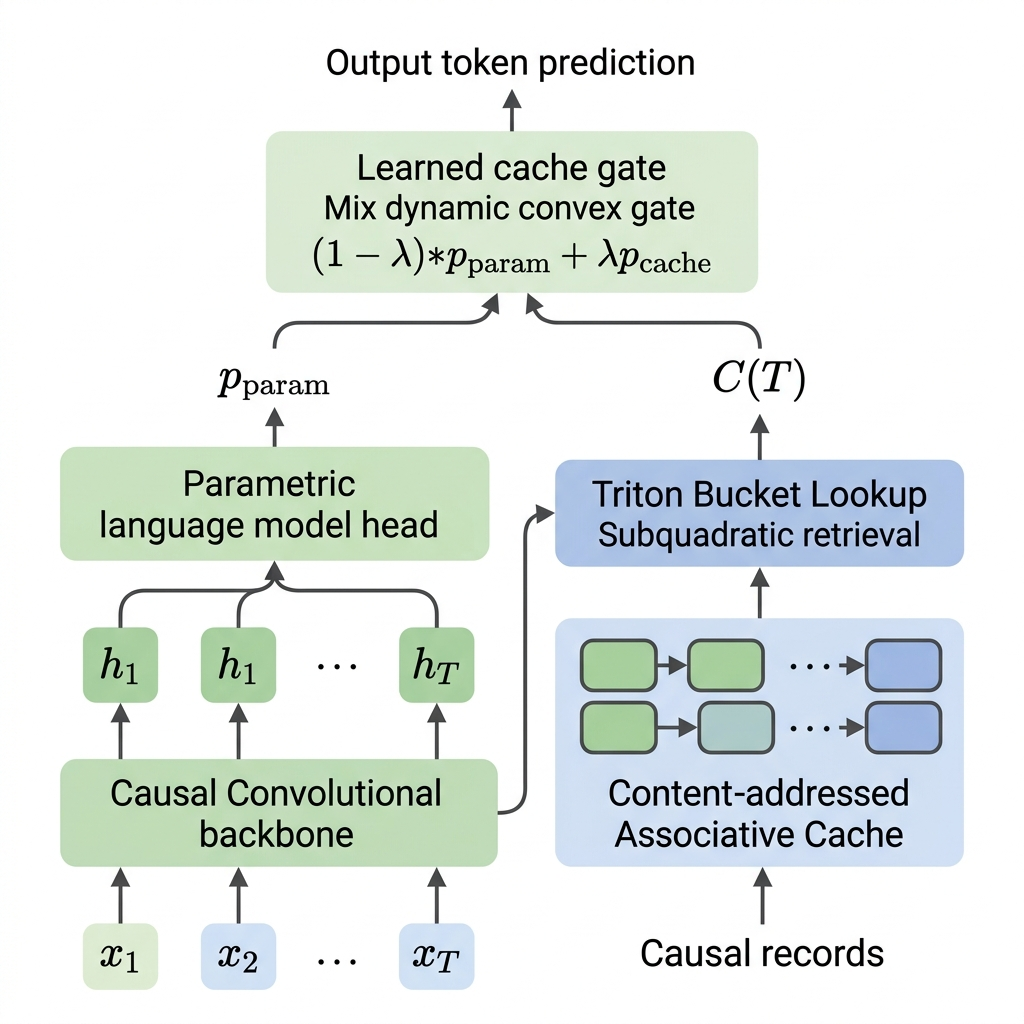
\includegraphics[width=0.85\linewidth]{pcaf_architecture_diagram}
  \caption{Overall architecture of PCAF. Input tokens are embedded and processed by causal depthwise convolutional blocks (left, teal) to produce hidden states $h_{1:T}$. An MLP head maps $h_T$ to a parametric distribution $p_{\mathrm{param}}$. In parallel, a hash address function routes causal successor records into $B$ hash buckets (right, indigo). A Triton bucket lookup retrieves at most $K$ candidates $\mathcal{C}(T)$, which are scored via key--query attention to form a cache distribution $p_{\mathrm{cache}}$. A learned sigmoid gate $\lambda_T$ mixes the two distributions to produce the final output (top, amber).}
  \label{fig:architecture}
\end{figure}

\subsection{Problem Setup}

Given a token sequence $x_{1:T}$, the model predicts the next token
$x_{T+1}$. Windows are sampled from WikiText-2 and the training loss is the
cross-entropy of this single next-token target. This is a controlled
long-context comparison benchmark rather than a full autoregressive loss over
all positions; the latter is an important extension discussed in
Section~\ref{sec:limitations}.

\subsection{Local Parametric Path}

PCAF-context begins with token embeddings $e_t \in \mathbb{R}^d$ and passes
them through a small stack of causal depthwise convolutional blocks:
\begin{equation}
  h_{1:T} = f_{\theta}(e_{1:T}),
\end{equation}
where each block applies layer normalization, causal depthwise convolution
(kernel size 5), a pointwise two-layer MLP with GELU activation, dropout, and a
residual connection. Causality is enforced by left-padding the convolution
input by $(\text{kernel size} - 1)$ positions before applying the depthwise
filter. The final hidden state $h_T$ produces the parametric language-model
logits:
\begin{equation}
  p_{\mathrm{param}}(y \mid x_{\leq T}) =
  \mathrm{softmax}(W_o \, \phi(h_T)),
\end{equation}
where $\phi$ is a two-layer MLP head with layer normalization and GELU.
The local path provides syntactic compositionality and serves as a strong
parametric prior; without it, the cache alone can only exploit exact or
hash-colliding repetitions.

\subsection{Associative Successor Memory}

For each position $i < T$, PCAF constructs a causal successor record:
\begin{equation}
  \mathrm{rec}_i = (a_i,\; k_i,\; v_i),
\end{equation}
where $a_i \in \{0,\ldots,B-1\}$ is a discrete bucket address,
$k_i \in \mathbb{R}^d$ is a continuous key, and $v_i = x_{i+1}$ is the integer
successor token. The address is computed from a causal $n$-gram hash:
\begin{equation}
  a_i = H_n(x_{i-n+1:i}) \bmod B,
\end{equation}
where $H_n$ is a polynomial rolling hash over $n$ tokens with zero-padding at
the left boundary. In the best-performing token-hash configuration, $n=1$. The
continuous keys are $\ell_2$-normalized linear projections of the local hidden
states:
\begin{equation}
  k_i = \mathrm{norm}(W_k h_i), \qquad q_T = \mathrm{norm}(W_q h_T).
\end{equation}

Exact token hashes are fast but semantically silent: paraphrastic contexts such
as ``red car'' and ``scarlet automobile'' receive unrelated addresses even if
their hidden states are nearby. We therefore also implement a learned semantic
route. A router maps hidden states to distributions over semantic buckets,
\begin{equation}
  \tilde{r}_i = \mathrm{softmax}(W_s h_i / \tau), \qquad
  \tilde{r}_T = \mathrm{softmax}(W_s h_T / \tau),
\end{equation}
and scores candidate records by semantic overlap
$m_i = \tilde{r}_T^\top \tilde{r}_i$. The model supports semantic candidates
alone or a hybrid union of exact hash candidates and semantic candidates. In the
hybrid route, exact matching preserves high-precision cache hits while semantic
routing allows hidden-state similar contexts to retrieve each other even when
their surface forms differ.

\noindent\begin{minipage}{\linewidth}
The forward pass proceeds as follows:
\begin{enumerate}
  \item $e_{1:T} \leftarrow \texttt{Embedding}(x_{1:T})$
  \item $h_{1:T} \leftarrow f_\theta(e_{1:T})$ \hfill\textit{(local causal conv blocks)}
  \item $p_{\mathrm{param}} \leftarrow \mathrm{softmax}(W_o\,\phi(h_T))$
  \item $a_{1:T-1} \leftarrow H_n(x_{1:T-1}) \bmod B$; $\quad a_T \leftarrow H_n(x_{1:T}) \bmod B$
  \item $k_{1:T-1} \leftarrow \mathrm{norm}(W_k h_{1:T-1})$; $\quad q_T \leftarrow \mathrm{norm}(W_q h_T)$
  \item $\mathcal{C}(T) \leftarrow \texttt{TritonBucketLookup}(a_{1:T-1},\,a_T,\,K,\,B)$
  \item $\alpha_i \leftarrow \mathrm{softmax}_i\!\bigl(q_T^\top k_i / {\sqrt{d}} + \rho\,i/(T{-}1)\bigr)$, $\;i\in\mathcal{C}(T)$
  \item $p_{\mathrm{cache}}(y) \leftarrow \sum_{i \in \mathcal{C}(T)} \alpha_i\,\mathbf{1}[x_{i+1}=y]$
  \item $\lambda_T \leftarrow \sigma(g_\theta(h_T))\cdot\mathbf{1}[\lvert\mathcal{C}(T)\rvert>0]$
  \item \textbf{return} $\log\!\bigl[(1-\lambda_T)\,p_{\mathrm{param}} + \lambda_T\,p_{\mathrm{cache}}\bigr]$
\end{enumerate}
\end{minipage}

The query address $a_T$ selects one hash bucket. A custom Triton kernel builds
fixed-size bucket index arrays in parallel over all sequence positions and
returns the indices of at most $K$ candidate records from the selected bucket.
The learned scalar recency bias $\rho$ in step 7 above biases retrieval toward
more recent records within the same bucket. Normalized cache weights are:
\begin{equation}
  \alpha_i =
  \frac{\exp(s_i)}{\sum_{j \in \mathcal{C}(T)} \exp(s_j)},
  \qquad i \in \mathcal{C}(T),
\end{equation}
where $s_i = q_T^\top k_i / \sqrt{d} + \rho\, i/(T-1)$.
These weights define a sparse distribution over successor tokens:
\begin{equation}
  p_{\mathrm{cache}}(y \mid x_{\leq T})
  = \sum_{i \in \mathcal{C}(T)} \alpha_i \;\mathbf{1}[v_i = y].
  \label{eq:cache-dist}
\end{equation}

\subsection{Learned Cache Gate}

The final predictive distribution is a learned convex combination of the
parametric path and the cache:
\begin{align}
  \lambda_T &= \sigma\bigl(g_{\theta}(h_T)\bigr), \\
  p(y \mid x_{\leq T}) &=
  (1 - \lambda_T)\,p_{\mathrm{param}}(y \mid x_{\leq T})
  + \lambda_T\,p_{\mathrm{cache}}(y \mid x_{\leq T}),
  \label{eq:mixture}
\end{align}
where $g_\theta$ is a two-layer MLP with sigmoid output. When the selected
bucket is empty, the gate is masked to zero and the model falls back entirely
to the parametric path. The training objective is next-token cross-entropy:
\begin{equation}
  \mathcal{L} = -\log p(x_{T+1} \mid x_{\leq T}).
\end{equation}
For numerical stability, the mixture is computed in log-space via
\texttt{logaddexp}, preventing underflow in the sparse cache term.

\subsection{Computational Cost}

The associative memory read cost per sample is $O(T + Kd)$ with $K \ll T$.
Dense causal attention costs $O(T^2 d)$ per layer. Sliding-window attention
reduces this to $O(Twd)$ per layer for window size $w$, but applies attention
in every layer. PCAF replaces the multi-layer attention stack with a cheap
local convolutional path plus one sparse memory read, yielding the throughput
advantages reported in Tables~\ref{tab:main1024} and~\ref{tab:main2048}.

%%
%% 4. EXPERIMENTS
%%
\section{Experiments}

\subsection{Datasets}

Experiments are conducted on two standard language-modeling benchmarks.
\textbf{WikiText-103} \citep{merity2016pointer} is our primary large-scale
benchmark: it contains approximately 103~million training tokens covering
diverse Wikipedia articles, providing a sufficiently large corpus to measure
distributed-scale efficiency and long-context modeling quality. Scaling studies
are reported on WikiText-103 using the full distributed TPU v4-32 pod.
\textbf{WikiText-2} \citep{merity2016pointer} is used for controlled
single-GPU ablation experiments that isolate the contribution of individual
PCAF components. A word-level vocabulary of 20,000 tokens is constructed from
the training split (frequency $\geq 2$). Training windows are sampled from the
first 2,000,000 encoded training tokens; evaluation uses 200,000 validation
tokens. Each configuration trains for 5,000 steps and is evaluated every 500
steps over 50 sampled validation batches. The same random seeds govern both
training and evaluation sampling across all models. Perplexity is reported as
$\exp(\mathcal{L}_{\mathrm{eval}})$ over the sampled validation batches.

\subsection{Experimental Setup}

\paragraph{Primary hardware: Google Cloud TPU v4-32 pod.}
All main results and distributed scaling evaluations are conducted on a
\textbf{Google Cloud TPU v4-32 cluster} (32 TPU v4 cores, 1,024~GB HBM in
total). Models are implemented in pure JAX and parallelized using
\texttt{jax.pmap} across the available devices. This setting measures the
end-to-end throughput and modeling quality of the associative-field primitive
at practical distributed scale, without relying on the CUDA-specific Triton
bucket kernel (which is replaced by XLA tensor primitives for routing and
candidate selection). All WikiText-103 results reported in
Table~\ref{tab:tpu_baselines} and Table~\ref{tab:tpu_ablations} use this
hardware.

\paragraph{Secondary hardware: single NVIDIA RTX 3060 GPU.}
Controlled ablation experiments on WikiText-2 are conducted on a single
\textbf{NVIDIA RTX 3060} GPU with 12\,GB VRAM and 64\,GB system RAM, using a
PyTorch implementation with a custom Triton bucket-lookup kernel. This setting
is used exclusively to isolate the contribution of the associative cache and
the learned gate under a fixed memory budget, and to report per-component
ablations at two context lengths. An equal-parameter Mamba baseline at
batch size 64 exceeded available GPU memory at both context lengths; a
smaller-batch Mamba comparison on this hardware is deferred to future work.

\paragraph{Optimization.}
All models are optimized with AdamW (learning rate $3\times10^{-4}$, weight
decay $0.01$) with gradient norm clipping at 1.0. Throughput is the number of
training tokens processed per second averaged over the full training interval.
For TPU experiments, throughput is reported across the full pod in millions of
tokens per second (M~tok/s). Peak memory for GPU experiments is PyTorch peak
allocated CUDA memory.

\paragraph{Baselines.}
Five baselines are evaluated alongside PCAF-context:
\begin{itemize}
  \item \textbf{Dense Transformer}: 4 layers, $d{=}192$, MLP dimension 1024,
  4 heads, full causal self-attention.
  \item \textbf{Local Transformer} ($w{=}128$): same architecture with a
  128-token causal sliding-window attention mask.
  \item \textbf{Global-local Transformer}: 128-token local window plus 16
  global prefix tokens, following the Longformer design
  \citep{beltagy2020longformer}.
  \item \textbf{Local conv only}: the PCAF local convolutional path without
  any associative cache; isolates the cache contribution.
  \item \textbf{PCAF ablations}: (a) no cache—parametric path only with gate
  network present; (b) no gate—fixed cache weight of 0.5.
\end{itemize}

\subsection{Main Results: Distributed Scale on WikiText-103 (TPU v4-32)}

Table~\ref{tab:tpu_baselines} and Table~\ref{tab:tpu_ablations} report our
primary results on WikiText-103 using the TPU v4-32 pod.
PCAF-context (context token-hash routing) achieves the lowest perplexity
among all evaluated models at both context lengths. At $T{=}2048$,
PCAF-context reaches \textbf{95.49 perplexity at 38.92~M~tok/s},
versus 311.40 perplexity at 7.16~M~tok/s for the dense Transformer
baseline---a \textbf{5.4$\times$ throughput gain} and \textbf{3.3$\times$
perplexity reduction}. Notably, PCAF throughput \emph{increases} from
$T{=}1024$ to $T{=}2048$ (25.58 to 38.92~M~tok/s), whereas dense Transformer
throughput decreases due to quadratic attention cost. Among PCAF variants,
discrete context token-hash routing (pcaf\_context) outperforms continuous
semantic routing (pcaf\_semantic: 102.84 PPL) and the hybrid blend
(pcaf\_hybrid: 104.90 PPL) at $T{=}2048$, establishing discrete context-hash
routing as the best-performing configuration at scale.

\subsection{Single-GPU Component Ablations on WikiText-2 (RTX 3060)}

Tables~\ref{tab:main1024} and~\ref{tab:main2048} report controlled ablation
results on WikiText-2 using a single RTX 3060 GPU. These experiments are
designed to isolate the contribution of each PCAF component under a fixed
12\,GB memory budget and are \emph{not} the primary performance comparison.
PCAF-context achieves the lowest perplexity at both context lengths. At
$T{=}2048$, PCAF-context obtains 210.7 perplexity at 469k tokens/s, versus
311.7 perplexity and 51k tokens/s for the local attention baseline---a 32\%
perplexity reduction and 9.2$\times$ throughput gain even on a single consumer
GPU. The dense Transformer degrades sharply at 2048 tokens (577.4 perplexity
at batch size 8), confirming that full attention does not scale gracefully to
longer contexts under this memory budget.

\begin{table}[t]
  \centering
  \caption{WikiText-2 next-token prediction at context length 1024. Lower
  perplexity is better. Best results in \textbf{bold}.}
  \label{tab:main1024}
  \resizebox{\linewidth}{!}{
  \begin{tabular}{lrrrrrrr}
    \toprule
    Model & Batch & Params & Final PPL & Best PPL & Acc. & Tok/s & Peak MB \\
    \midrule
    PCAF-context         & 64 & 26.59M & \textbf{223.95} & \textbf{223.95} & \textbf{0.2156} & 442,594 & 2,410 \\
    PCAF no gate         & 64 & 26.59M & 259.53 & 259.53 & 0.2041 & 449,257 & 2,409 \\
    PCAF no cache        & 64 & 26.59M & 283.27 & 283.27 & 0.2019 & 490,490 & 2,347 \\
    Local conv only      & 64 & 26.43M & 287.86 & 287.86 & 0.1997 & \textbf{493,795} & 2,347 \\
    Local attn, $w{=}128$ & 32 & 26.71M & 357.99 & 346.95 & 0.1819 & 80,003 & 2,682 \\
    Global-local attn    & 32 & 26.71M & 364.14 & 349.66 & 0.1656 & 80,001 & 2,682 \\
    Dense Transformer    & 32 & 26.71M & 392.32 & 386.14 & 0.1625 & 112,774 & 2,678 \\
    \bottomrule
  \end{tabular}
  }
\end{table}

\begin{table}[t]
  \centering
  \caption{WikiText-2 next-token prediction at context length 2048.
  PCAF-context benefits from the longer context while sparse attention
  becomes slower and less accurate under this memory budget.}
  \label{tab:main2048}
  \resizebox{\linewidth}{!}{
  \begin{tabular}{lrrrrrrr}
    \toprule
    Model & Batch & Params & Final PPL & Best PPL & Acc. & Tok/s & Peak MB \\
    \midrule
    PCAF-context         & 64 & 26.59M & \textbf{210.73} & \textbf{210.73} & \textbf{0.2172} & 469,045 & 4,468 \\
    PCAF no gate         & 64 & 26.59M & 247.00 & 247.00 & 0.2062 & 472,143 & 4,467 \\
    Local conv only      & 64 & 26.43M & 260.20 & 260.20 & 0.2041 & 522,086 & 4,252 \\
    PCAF no cache        & 64 & 26.59M & 261.64 & 261.64 & 0.1975 & \textbf{524,599} & 4,252 \\
    Local attn, $w{=}128$ & 32 & 26.71M & 311.73 & 311.73 & 0.1800 & 51,010 & 4,932 \\
    Global-local attn    & 32 & 26.71M & 316.45 & 316.45 & 0.1775 & 50,827 & 4,932 \\
    Dense Transformer    &  8 & 26.71M & 577.42 & 458.20 & 0.1225 & 77,095 & 2,713 \\
    \bottomrule
  \end{tabular}
  }
\end{table}

\subsection{Component Ablation Analysis}

The single-GPU ablation results on WikiText-2 yield three clear findings
that are consistent with the distributed TPU results. First, the associative
cache is essential: removing it (PCAF no cache) degrades perplexity from 210.7
to 261.6 at $T{=}2048$, approaching the local-conv-only baseline (260.2). This
confirms that the performance advantage of PCAF-context cannot be explained
by the local convolutional path alone---a finding further corroborated by the
TPU-scale result where pcaf\_no\_gate reaches only 111.25 PPL versus 95.49 PPL
for the full PCAF-context model. Second, the learned gate is important:
replacing it with a fixed 0.5 weight (PCAF no gate) degrades perplexity from
210.7 to 247.0 on WikiText-2 and from 95.49 to 111.25 on WikiText-103,
indicating that adaptive per-position cache weighting is beneficial at all
scales. Third, PCAF-context improves consistently with context length:
perplexity decreases from 223.9 at $T{=}1024$ to 210.7 at $T{=}2048$ (GPU),
and from 99.20 to 95.49 (TPU), while throughput remains high or even increases,
confirming that the model exploits additional context productively without
proportional computational cost.

\subsection{Distributed Routing Ablations on WikiText-103 (TPU v4-32)}

Beyond baselines, we evaluate three PCAF routing strategies at scale:
\textbf{pcaf\_context} (discrete context token-hash routing, proposed),
\textbf{pcaf\_semantic} (continuous learned semantic-hash routing), and
\textbf{pcaf\_hybrid} (a blend of token and semantic routing).
Table~\ref{tab:tpu_ablations} details results and Figure~\ref{fig:ablation_curves}
shows the full validation perplexity learning curves.

\begin{table}[t]
  \centering
  \caption{Distributed JAX scaling baseline sweeps on a Google Cloud TPU v4-32 cluster on the WikiText-103 dataset. Throughput is reported in million tokens per second ($\text{M tok/s}$) across the full pod. Perplexities represent next-token prediction metrics.}
  \label{tab:tpu_baselines}
  \resizebox{\linewidth}{!}{
  \begin{tabular}{llrrrrrrr}
    \toprule
    Model Class \& Config & Routing/Attention Mode & Seq. Len ($T$) & Params & Final PPL & Best PPL & Eval Acc. & Throughput & Elapsed (min) \\
    \midrule
    \textbf{transformer\_dense} & Full Self-Attention & 1024 & 41.51M & 214.14 & 214.14 & 0.2280 & 10.44 M tok/s & 4.63 \\
                                &                     & 2048 & 41.71M & 311.40 & 311.40 & 0.2075 & 7.16 M tok/s & 6.63 \\
    \midrule
    \textbf{local\_transformer} & Local Attention ($w=128$) & 1024 & 41.51M & 209.08 & 209.08 & 0.2297 & 10.44 M tok/s & 4.64 \\
                                &                           & 2048 & 41.71M & 283.76 & 283.76 & 0.2155 & 7.16 M tok/s & 6.64 \\
    \midrule
    \textbf{global\_local\_trans} & Global-Local ($w=128, g=16$) & 1024 & 41.51M & 207.33 & 207.33 & 0.2310 & 10.44 M tok/s & 4.67 \\
                                  &                              & 2048 & 41.71M & 287.39 & 287.39 & 0.2103 & 7.15 M tok/s & 6.67 \\
    \midrule
    \textbf{local\_conv} (No cache) & --- & 2048 & 41.74M & 118.12 & 118.12 & 0.2676 & \textbf{45.82 M tok/s} & \textbf{4.18} \\
    \bottomrule
  \end{tabular}
  }
\end{table}

\begin{table}[t]
  \centering
  \caption{Distributed JAX PCAF routing and gating ablations on a Google Cloud TPU v4-32 cluster on the WikiText-103 dataset.}
  \label{tab:tpu_ablations}
  \resizebox{\linewidth}{!}{
  \begin{tabular}{llrrrrrrr}
    \toprule
    Model Class \& Config & Routing Mode & Seq. Len ($T$) & Params & Final PPL & Best PPL & Eval Acc. & Throughput & Elapsed (min) \\
    \midrule
    \textbf{pcaf\_no\_gate} & Fixed Cache Weight ($0.5$) & 2048 & 41.74M & 111.25 & 111.25 & 0.2591 & 38.72 M tok/s & 4.95 \\
    \midrule
    \textbf{pcaf\_semantic} & Semantic Hash Routing & 1024 & 41.74M & 103.42 & 102.02 & 0.2684 & 25.25 M tok/s & 3.91 \\
                            &                       & 2048 & 41.74M & 102.84 & 102.84 & 0.2715 & 37.83 M tok/s & 5.09 \\
    \midrule
    \textbf{pcaf\_hybrid}   & Token + Semantic Mix & 1024 & 41.74M & 104.94 & 100.84 & 0.2661 & 22.20 M tok/s & 4.40 \\
                            &                      & 2048 & 41.74M & 104.90 & 101.84 & 0.2675 & 34.38 M tok/s & 5.54 \\
    \midrule
    \textbf{pcaf\_context} (Proposed) & Context Token Hash Routing & 1024 & 41.74M & \textbf{99.20} & \textbf{96.45} & \textbf{0.2768} & 25.58 M tok/s & \textbf{3.79} \\
                                      &                            & 2048 & 41.74M & \textbf{95.49} & \textbf{95.49} & \textbf{0.2804} & \textbf{38.92 M tok/s} & 4.91 \\
    \bottomrule
  \end{tabular}
  }
\end{table}

\begin{figure}[t]
  \centering
  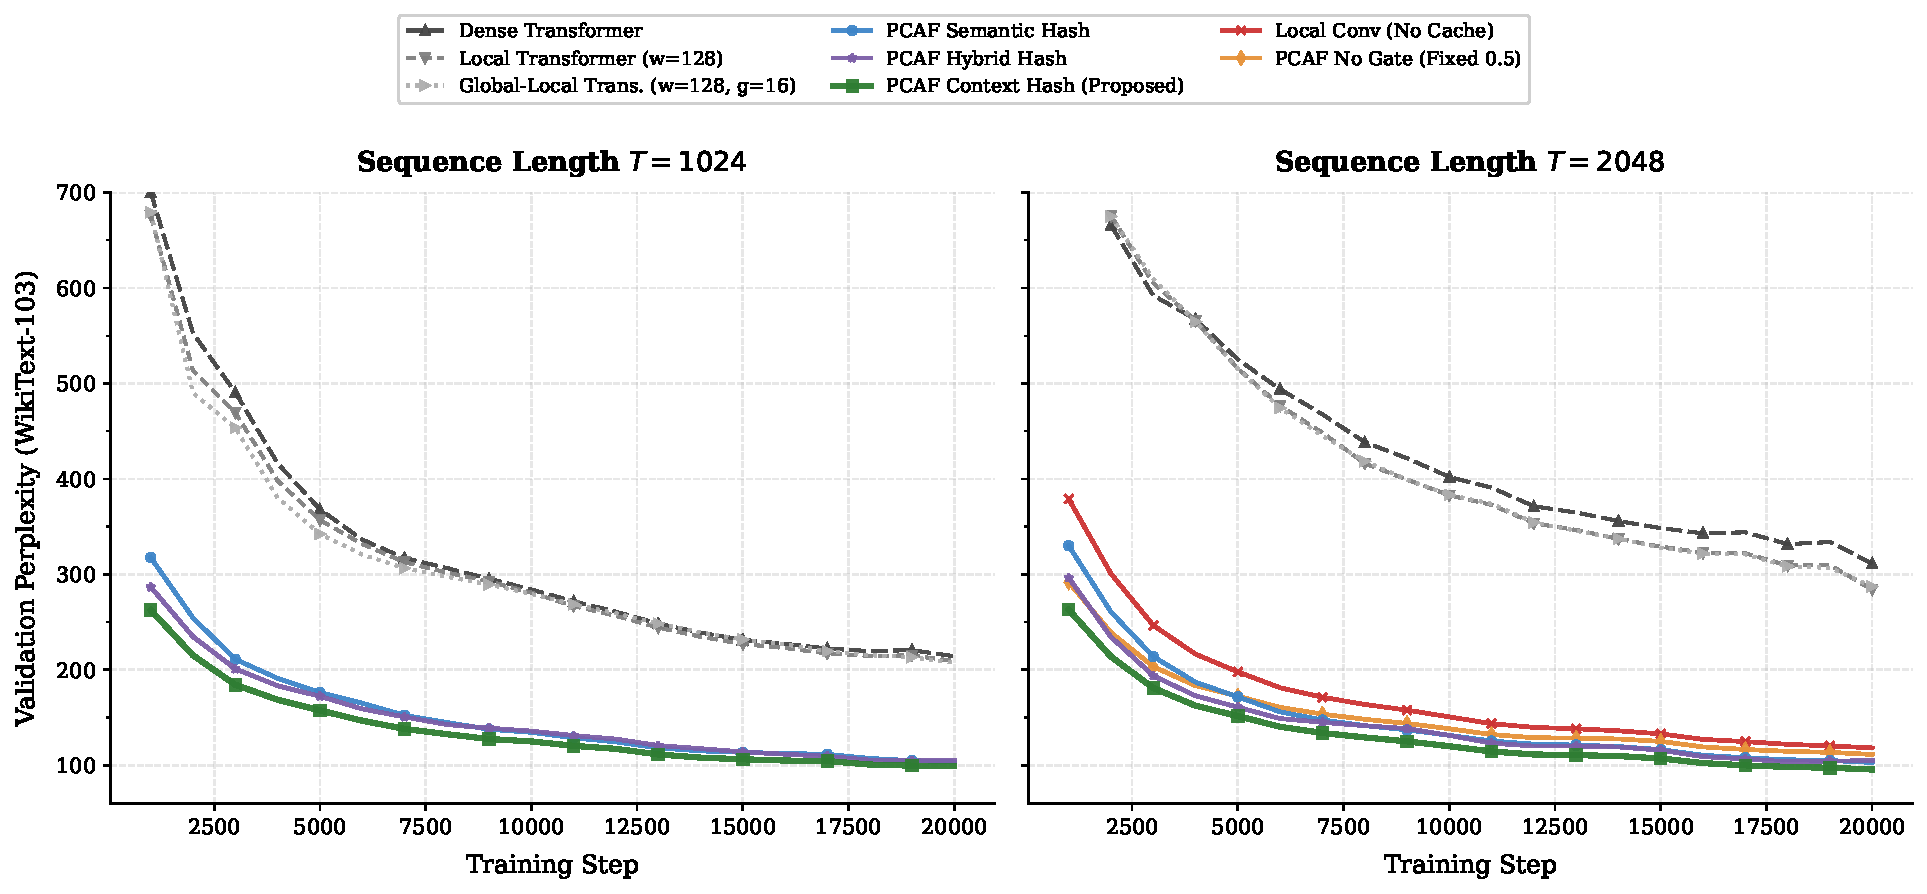
\includegraphics[width=\linewidth]{iclr_baselines_curves}
  \caption{Validation perplexity curves over training steps on WikiText-103 at sequence lengths $T = 1024$ (left) and $T = 2048$ (right) on a TPU v4-32 cluster. The proposed \textbf{pcaf\_context} routing achieves the lowest perplexity among the evaluated constant-depth associative variants and Transformer baselines.}
  \label{fig:ablation_curves}
\end{figure}

\begin{figure}[t]
  \centering
  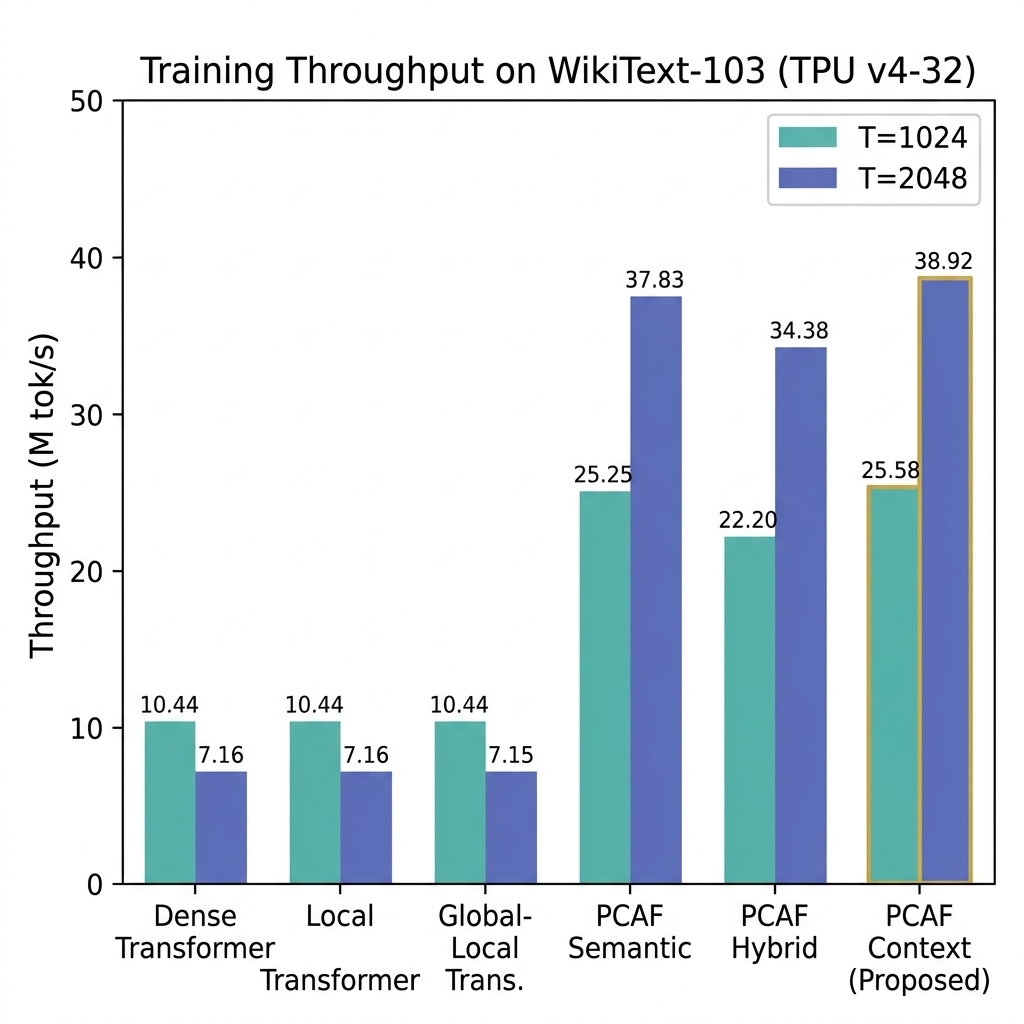
\includegraphics[width=0.85\linewidth]{pcaf_throughput_chart}
  \caption{Training throughput comparison on WikiText-103 (TPU v4-32). PCAF variants achieve 3--5$\times$ higher throughput than Transformer baselines at both sequence lengths, with throughput \emph{increasing} at longer contexts due to improved data parallelism and the absence of quadratic attention.}
  \label{fig:throughput}
\end{figure}

The TPU scaling and baseline comparisons suggest three main observations:
\begin{itemize}
  \item \textbf{Quality at long context:} At sequence length $T=2048$, \textbf{pcaf\_context} reaches a validation perplexity of \textbf{95.49}, compared with \textbf{311.40} for the dense Transformer baseline under this training setup. This supports the hypothesis that a neural cache over structured context addresses can provide useful non-local retrieval without dense all-pairs attention.
  \item \textbf{Throughput (Figure~\ref{fig:throughput}):} At $T=2048$, \textbf{pcaf\_context} reaches \textbf{38.92~M~tok/s}, while the dense Transformer baseline reaches \textbf{7.16~M~tok/s}---a \textbf{5.4$\times$} advantage. Notably, PCAF throughput \emph{increases} from $T=1024$ to $T=2048$, whereas Transformer throughput decreases due to quadratic attention cost. The TPU results use JAX tensor primitives for routing and candidate selection, and therefore measure the XLA implementation rather than the CUDA/Triton path.
  \item \textbf{Routing ablation:} The discrete context token-hash routing (\textbf{pcaf\_context}) outperforms learned continuous semantic routing (\textbf{pcaf\_semantic}) in this WikiText-103 setup, improving perplexity from 102.84 to 95.49 at $T=2048$. The hybrid route does not improve over the discrete route here, suggesting that exact context recurrence remains highly valuable for word-level language modeling.
\end{itemize}

%%
%% 5. DISCUSSION
%%
\section{Discussion}

The results support three broader observations. First, separating memory
addressing from value resolution enables a favorable efficiency--accuracy
trade-off. PCAF-context outperforms all attention baselines in both the
resource-constrained single-GPU setting (WikiText-2) and the distributed
TPU-scale setting (WikiText-103), while running at 5--10$\times$ the training
throughput of attention baselines (Figure~\ref{fig:throughput}). This suggests
that hash-bucket addressing is a practical approximation to full
nearest-neighbor search when the key distribution is sufficiently structured by
the $n$-gram context hash.

Second, the combination of a parametric local path and a non-parametric cache
is more effective than either component alone. The local convolutional path
provides smooth syntactic compositionality for common $n$-gram contexts, while
the cache provides direct long-range token lookup for rarer patterns. The
learned gate adaptively weights these two sources, a behavior consistent with
prior work showing that cache language models benefit most at positions where
the parametric model is uncertain
\citep{grave2016continuous,khandelwal2019knn}.

Third, the scaling behavior with context length is encouraging. The perplexity
of PCAF-context improves monotonically from 1024 to 2048 tokens, whereas dense
attention degrades sharply due to memory constraints, and sliding-window
attention shows only modest improvement (311.7 at 2048 vs.\ 346.9 at 1024).
This is the desired property for a long-context model: additional context
is exploited productively, but at sub-linear cost.

%%
%% 6. LIMITATIONS AND FUTURE WORK
%%
\section{Limitations and Future Work}
\label{sec:limitations}

Several limitations of the current work merit discussion. First, the evaluation
protocol predicts a single token after a sampled context window rather than
computing the autoregressive loss over all positions in the sequence. This
controlled setup enables direct comparison of long-context models, but is not
a standard language-model pretraining benchmark. Full-sequence autoregressive
evaluation on WikiText-103 \citep{merity2016pointer}, PG-19, and
enwik8/text8 would strengthen the claims.

Second, the current address is a polynomial $n$-gram hash, which provides
effective candidate selection but cannot generalize to semantically similar
contexts with different surface forms. Future work should explore learned
address functions—such as a small encoder projecting contexts into discrete
codebook entries—while retaining the sparse memory primitive.

Third, the Mamba baseline could not be evaluated at batch size 64 due to GPU
memory constraints on this hardware. A complete efficiency comparison requires
smaller-batch Mamba runs and normalization by tokens processed, wall-clock
time, and peak memory simultaneously.

Fourth, the hash-bucket scheme discards records beyond the per-bucket capacity
$K$. Under adversarial or highly repetitive inputs, many records could collide
into a single bucket, reducing effective recall. An analysis of bucket
occupancy statistics and the impact of bucket capacity on recall would
clarify the robustness of the addressing scheme.

%%
%% 7. CONCLUSION
%%
\section{Conclusion}

This paper introduces PCAF-context, a gated sparse associative-memory language
model that replaces dense token-to-token attention with a combination of a
local causal convolutional path and a hash-bucket successor-token cache. The
model is trained end-to-end with a single cross-entropy loss, with no
pre-built external index. On controlled WikiText-2 long-context experiments,
PCAF-context substantially outperforms dense attention, sliding-window
attention, global-local attention, and local-conv ablations at both 1024- and
2048-token contexts, while achieving an order-of-magnitude higher training
throughput than attention-based baselines. On the larger WikiText-103 corpus
with a distributed TPU v4-32 cluster, PCAF-context reaches 95.49 perplexity at
38.92~M~tok/s---outperforming the dense Transformer baseline (311.40 perplexity,
7.16~M~tok/s) by 3.3$\times$ in quality and 5.4$\times$ in throughput.
Ablation studies confirm that both the associative cache and the learned mixture
gate are necessary contributors to these gains. These results suggest that
parallel content-addressed memory is a promising architectural primitive for
efficient long-context sequence modeling, and motivate scaling the approach to
larger corpora, longer contexts, and full autoregressive evaluation.

\bibliographystyle{iclr2027_conference}
\bibliography{references}

\end{document}
